\documentclass{article}
\usepackage{amsmath}
\usepackage{fontspec}
\usepackage{xunicode}
\usepackage{indentfirst}
% add algorithm
\usepackage{algorithm}  
\usepackage{algorithmic}
\usepackage{graphicx}  
% from denny
\usepackage[utf8]{inputenc}
\usepackage{amssymb}
\usepackage{subfig}
\usepackage{bbm}

\usepackage[dvipsnames,svgnames]{xcolor}
% \usepackage[usenames, dvipsnames]{color}
% \definecolor{mypink2}{RGB}{219, 48, 122}
% \definecolor{mypink3}{cmyk}{0, 0.7808, 0.4429, 0.1412}

\colorlet{LightRubineRed}{RubineRed!70!}
\colorlet{Mycolor1}{green!10!orange!90!}
\definecolor{Mycolor2}{HTML}{00F9DE}

% \pagecolor{black}
% \color{white}
% alert 
\usepackage{environ}
% \usepackage{xcolor}
\usepackage[tikz]{bclogo,rotating}
\usepackage{tikz}
\usetikzlibrary{calc}
\usepackage{lipsum}
\DeclareGraphicsRule{.mps}{eps}{.mps}{}
 
\NewEnviron{myremark}[1]
  {\par\medskip\noindent
  \begin{tikzpicture}
    \node[inner sep=0pt] (box) {\parbox[t]{.99\textwidth}{%
      \begin{minipage}{.3\textwidth}
      \centering\tikz[scale=5]\node[scale=3,rotate=30]{\bclampe};
      \end{minipage}%
      \begin{minipage}{.65\textwidth}
      \textbf{#1}\par\smallskip
      \BODY
      \end{minipage}\hfill}%
    };
    \draw[red!75!black,line width=3pt]
      ( $ (box.north east) + (-5pt,3pt) $ ) -- ( $ (box.north east) + (0,3pt) $ ) -- ( $ (box.south east) + (0,-3pt) $ ) -- + (-5pt,0);
    \draw[red!75!black,line width=3pt]
      ( $ (box.north west) + (5pt,3pt) $ ) -- ( $ (box.north west) + (0,3pt) $ ) -- ( $ (box.south west) + (0,-3pt) $ ) -- + (5pt,0);
  \end{tikzpicture}\par\medskip%
}

\graphicspath{ {pic/} }

%% XeTeX adds code when switching latin (0) or boundary (255) to CJK (1, 2, 3)
\XeTeXinterchartokenstate = 1

%% Fonts for Latin and CJK
\newfontfamily\rmfont{TeX Gyre Pagella}
\newfontfamily\cjkfont{SimSun}

%% Ranges for Latin Font
\XeTeXinterchartoks 1 0 = {\rmfont}
\XeTeXinterchartoks 2 0 = {\rmfont}
\XeTeXinterchartoks 3 0 = {\rmfont}
\XeTeXinterchartoks 255 0 = {\rmfont}

%% Ranges for CJK Font
\XeTeXinterchartoks 0 1 = {\cjkfont}
\XeTeXinterchartoks 0 2 = {\cjkfont}
\XeTeXinterchartoks 0 3 = {\cjkfont}
\XeTeXinterchartoks 255 1 = {\cjkfont}
\XeTeXinterchartoks 255 2 = {\cjkfont}
\XeTeXinterchartoks 255 3 = {\cjkfont}

\XeTeXlinebreaklocale "zh"
\XeTeXlinebreakskip = 0pt plus 1pt

\DeclareMathOperator*{\argmin}{arg\,min}

\begin{document}
%%%%%%%%%%%%%%%%%%%%%%%%%%%%%%%%%%%%%%%%%%%%%%%%%%%%%section 1
\section{What is Maching Learning}
\noindent
{\color{LightRubineRed} \rule{\linewidth}{1mm} }
让机器去学习。有时候规则很难定义,比如怎么定义什么是一颗树。而让机器通过数据学习就会使问题变简单了。可以让机器自动挖掘一些模式。\par
\subsection{Machine learning}: \par
improving some Performance measure with experience computed from Data. \par
use \textcolor{Mycolor1}{data} to compute hypothesis g that \textcolor{Mycolor1}{approximates} target f. \par

\begin{center}
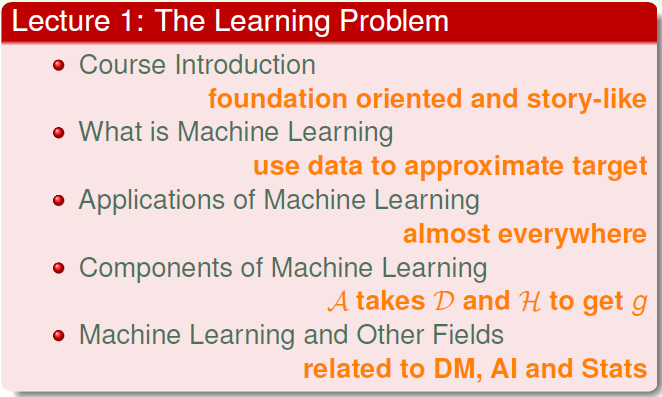
\includegraphics[width=10cm, height=6cm]{lecture1_sum}\\
\end{center}

\noindent
{\color{RubineRed} \rule{\linewidth}{1mm} }
% {\color{LightRubineRed} \rule{\linewidth}{1mm} }
%%%%%%%%%%%%%%%%%%%%%%%%%%%%%%%%%%%%%%%%%%%%%%%%%%%%%section 2
%%%%%%%%%%%%%%%%%%%%%%%%%%%%%%%%%%%%%%%%%%%%%%%%%%%%%section 2
\section{Learning to Answer Yes/No} % (fold)
\noindent
{\color{LightRubineRed} \rule{\linewidth}{1mm} }
\subsection{Perceptron}
\begin{align*}
h(x) &= sign((\sum_{i=1} W_i x_i - \text{threshold})) \\
     &= sign((\sum_{i=0} W_i x_i)) \\
     &= sign(W^TX)
\end{align*}
\begin{center}
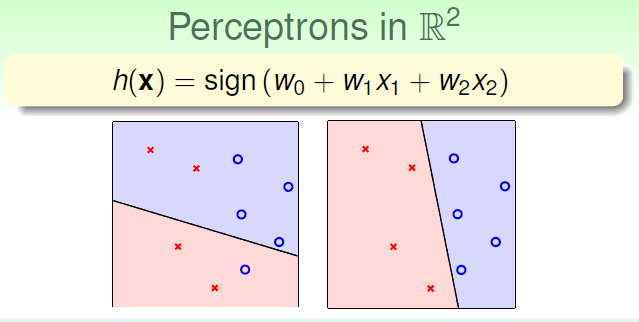
\includegraphics[width=10cm, height=5cm]{lecture2_1}\\
\end{center}
\begin{algorithm}  
\caption{Perceptron Learning Algorithm}  
\begin{algorithmic}  
\FOR{$t\gets1$ to $m$ }  
  \STATE Find a \textcolor{Mycolor1}{mistake} of $W_t$
  \STATE eg. $sign(W_{t}^{T}x_{n(t)}) \neq y_{n(t)}$ 
  \STATE $W_{t+1} \gets W_{t} + y_{n(t)}x_{n(t)}$ 
\ENDFOR
% \STATE return $W$(called W_{PLA})
\end{algorithmic}  
\end{algorithm}
缺点就是必须线性可分 Linear Separability \par
\begin{center}
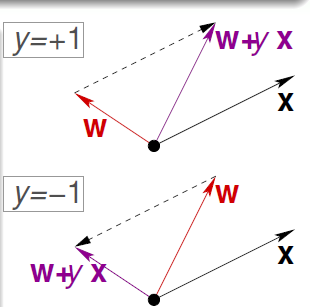
\includegraphics[width=5cm, height=5cm]{lecture2_2}\\
PLA \par
\end{center}
PLA Fact: $W_t$ Gets more Aligned with $W_f$,学习是能够保证$W$逐渐趋近于理想的$W_f$,
内积越大越相似。\par
\begin{align*}
w_f^{T}w_{t+1} &= w_f^{T}(w_t + y_{n(t)}x_{n(t)}) \\
               &\geq w_f^{T}w_t + \underset{n}{\min}y_nw_f^Tx_n \\
               &> w_f^Tw_t + 0.
\end{align*}
因此整个更新过程是$w_f \gets w_t$的,但有时候数据是有噪音的或者本身就不可分。 \par
% section section_name (end)
\begin{center}
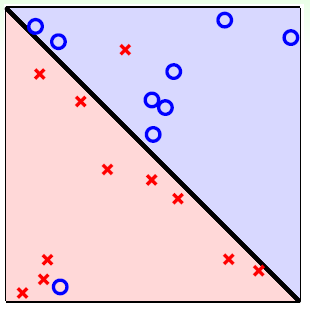
\includegraphics[width=5cm, height=5cm]{lecture2_3}\\
\end{center}
\subsection{Pocket}
\begin{algorithm}  
\caption{Pocket Algorithm}  
\begin{algorithmic}  
\STATE initialize pocket weights $\hat{w}$
\FOR{$t\gets1$ to $m$ }  
  \STATE 1.Find a \textcolor{Mycolor1}{mistake} of $W_t$
  \STATE eg. $sign(W_{t}^{T}x_{n(t)}) \neq y_{n(t)}$ 
  \STATE 2.$W_{t+1} \gets W_{t} + y_{n(t)}x_{n(t)}$ 
  \STATE 3.$W_{t+1} \gets \arg\underset{mistakes}{\min}(\hat{w},w_t)$
\ENDFOR
% \STATE return $W$(called W_{PLA})
\end{algorithmic}  
\end{algorithm}
\par
%%%%%%%%%%%%%%%%%%%%%Method one
\begin{bclogo}{Important!}
对PLA算法一个简单的修改(Pocket里永远是最好的),能处理有少许噪音的数据,但是速度要慢一点因为有比较的过程。 \par
\end{bclogo}
%%%%%%%%%%%%%%%%%%%%%Method tow
\begin{myremark}{Importance}
对PLA算法一个简单的修改(Pocket里永远是最好的),能处理有少许噪音的数据,但是速度要慢一点因为有比较的过程。 \par
\end{myremark}

\begin{center}
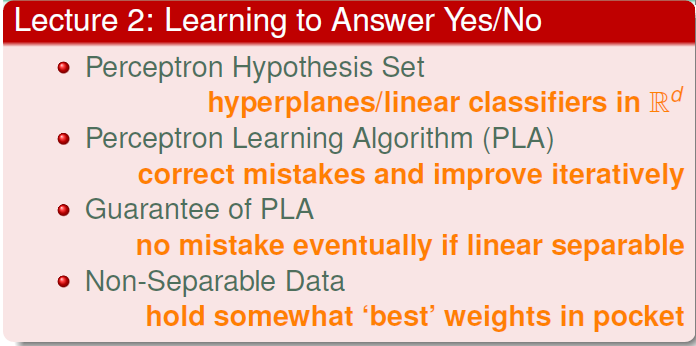
\includegraphics[width=10cm, height=5.5cm]{lecture2_sum}\\
\end{center}

\noindent
{\color{RubineRed} \rule{\linewidth}{1mm} }
%%%%%%%%%%%%%%%%%%%%%%%%%%%%%%%%%%%%%%%%%%%%%section 3
% \section{Types of Learning} % (fold)
% \noindent
% {\color{LightRubineRed} \rule{\linewidth}{1mm} }
% \begin{itemize}
% \item \textbf{Binary classification}:\par
% patient features $\Rightarrow$ sick or not 
% \begin{align}
% \mathcal{Y} = \{-1,+1\}
% \end{align}
% \item \textbf{Multiclass Classification}: \par
% pathent features $\Rightarrow$ which type of cancer 
% \begin{align}
% \mathcal{Y} = \{1,2,...,K\}
% \end{align}
% \item \textbf{regression}: \par
% pathent features $\Rightarrow$ how many days before recoverry 
% \begin{align}
% \mathcal{Y} = \mathbb{R}
% \end{align}
% \item \textbf{Sequence Learning}: \par
% NLP
% \end{itemize}
% \begin{center}
% 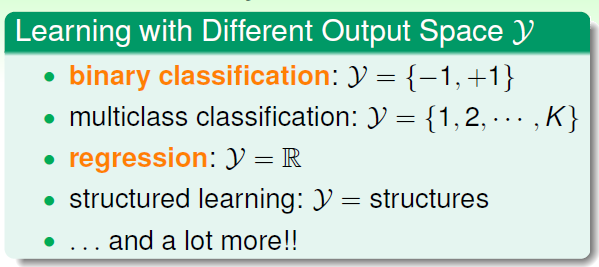
\includegraphics[width=10cm, height=5cm]{lecture3_1}\\
% \end{center}
% % section section_name (end)
% \noindent
% {\color{LightRubineRed} \rule{\linewidth}{1mm} }
% \begin{itemize}
% \item Supervised \par
% \item Unsupervised \par
% \item Semi-supervised \par
% \item Reinforcement
% \end{itemize}
% \begin{center}
% 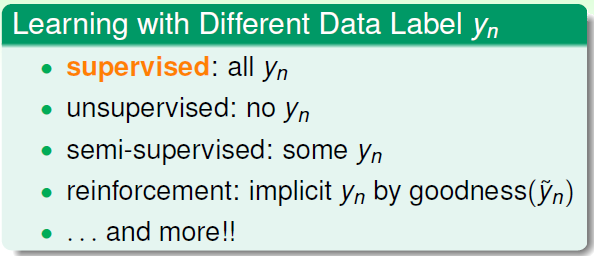
\includegraphics[width=10cm, height=4.5cm]{lecture3_2}\\
% \end{center}
% 输入,输出,训练模式,算法类型。
% \begin{center}
% 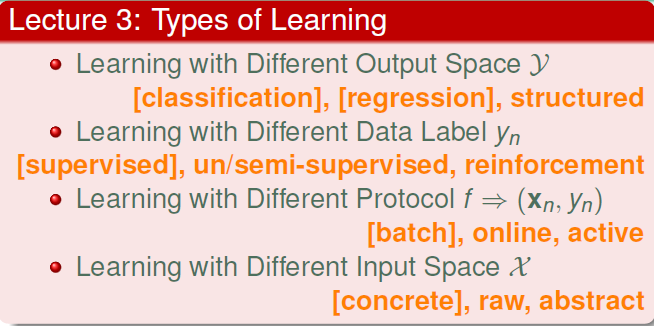
\includegraphics[width=10cm, height=5cm]{lecture3_sum}\\
% \end{center}
% \noindent
% {\color{RubineRed} \rule{\linewidth}{1mm} }
% %%%%%%%%%%%%%%%%%%%%%%%%%%%%%%%%%%%%%%%%%%%section 4
% \section{Feasibility of Learning}
% \noindent
% {\color{LightRubineRed} \rule{\linewidth}{1mm} }

% \subsection{No Free Lunch}
% Learning from $D$ (to infer something outside$D$) is doomed if any 'unknown' $f$ can happen. :( \par

% \subsection{Inferring something} % (fold)
% \begin{center}
% 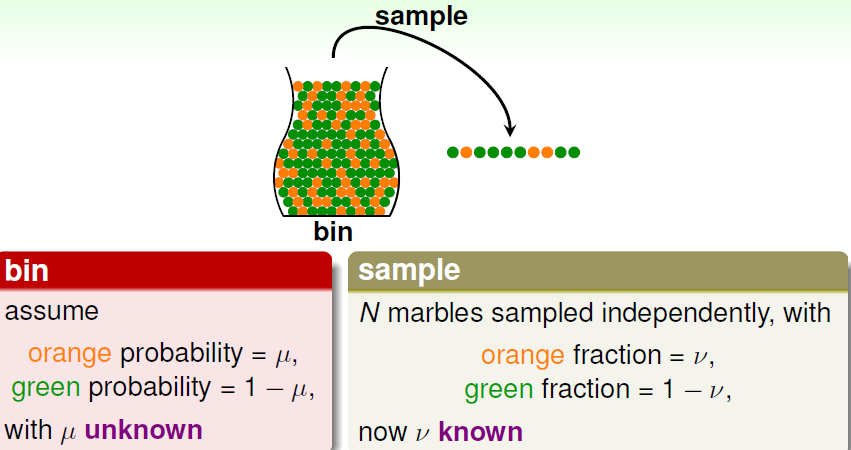
\includegraphics[width=10cm, height=6.5cm]{lecture4_1}\\
% \end{center}
% \textbf{Hoeffding's Inequality} \par
% \begin{align*}
% \mathbb{P}[|\nu-\mu| > \epsilon] \leq 2\exp(-2\epsilon^2N)
% \end{align*}
% 跟$\mu$无关,跟$N$有关,如果样本够多,大概可以去近似。 \par
% \subsection{Connection to Learning} % (fold)
% \begin{align*}
% E_{out}(h) &= \underset{x \sim P}{E} \llbracket h(x) \neq f(x) \rrbracket\\
% E_{in}(h) &= \frac{1}{N}\sum_{n=1}^N \llbracket h(x) \neq f(x) \rrbracket \\
% \end{align*}
% $E_{in}$out-of-sampling(Known) \\
% $E_{out}$in-of-sampling(UnKnown) \\
% 就像刚才一样我们不需要知道$E_{out}$,只需要$N$足够大即可。\par
% \begin{align*}
% \mathbb{P}[|E_{in}-E_{out}| > \epsilon] \leq 2\exp(-2\epsilon^2N)
% \end{align*}
% 这样从理论保证,对于固定的$h$,如果数据足够多的话。
% \begin{align*}
%   E_{in} \approx E_{out}
% \end{align*}
% \subsection{Multiple h} % (fold)
% Bound of Bad data \par
% %http://ccxxxx.blog.51cto.com/7769075/1339606
% \begin{align*}
% \mathbb{P}_D[\text{bad} \ \mathcal{D}] \\
% &= \mathbb{P}_D[\text{bad} \ \mathcal{D} \; for \; all \; h] \\
% &\leq 2M\exp{-2\epsilon^2N}
% \end{align*}
% 如果算法$A$找到一个$g$保证$E_{in} \approx 0$,那么理论保证$E_{out} \approx 0$ \\
% $M$应该代表了复杂度,$N$代表了数据多少,理解这两个数值对ML的优化很有帮助。 
% \begin{center}
% 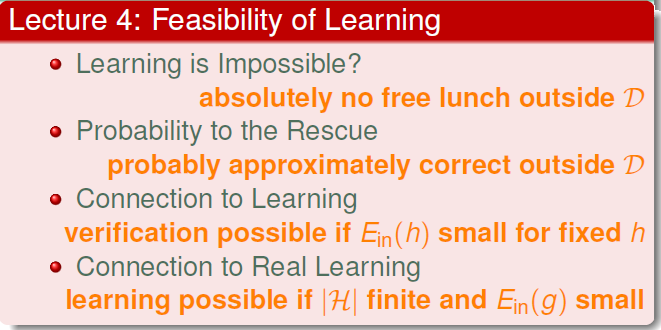
\includegraphics[width=10cm, height=6cm]{lecture4_sum}
% \end{center}
% \noindent
% {\color{RubineRed} \rule{\linewidth}{1mm} }
%%%%%%%%%%%%%%%%%%%%%%%%%%%%%%%%%%%%%
\end{document}